%%%%%%%%%%%%%%%%%%%%%%%%%%%%%%%%%%%%%%%%%
% Beamer Presentation
% LaTeX Template
% Version 1.0 (10/11/12)
%
% This template has been downloaded from:
% http://www.LaTeXTemplates.com
%
% License:
% CC BY-NC-SA 3.0 (http://creativecommons.org/licenses/by-nc-sa/3.0/)
%
%%%%%%%%%%%%%%%%%%%%%%%%%%%%%%%%%%%%%%%%%

%----------------------------------------------------------------------------------------
%	PACKAGES AND THEMES
%----------------------------------------------------------------------------------------

\documentclass[usenames,dvipsnames,table]{beamer}

\mode<presentation> {

\usetheme{Madrid}
%\setbeamertemplate{footline} % To remove the footer line in all slides uncomment this line
%\setbeamertemplate{footline}[page number] % To replace the footer line in all slides with a simple slide count uncomment this line
\setbeamertemplate{navigation symbols}{} % To remove the navigation symbols from the bottom of all slides uncomment this line
}

\usepackage{amsmath}
\usepackage{graphicx} % Allows including images
\usepackage{booktabs} % Allows the use of \toprule, \midrule and \bottomrule in tables
\usepackage{listings}
\usepackage{xcolor}
\usepackage{xfrac}
% \usepackage{enumitem}

\usefonttheme[onlymath]{serif}

%----------------------------------------------------------------------------------------
%	TITLE PAGE
%----------------------------------------------------------------------------------------

\title[ABDA Ch 15]{Applied Bayesian Data Analysis --- Chapter 15}

\author{Kim Albertsson} % Your name
\institute[LTU and CERN]
{
CERN and Luleå University of Technology \\
\medskip
\textit{kim.albertsson@ltu.se}
}
\date{\today}

\newcommand{\cgy}{\cellcolor{gray!25}}
\newcommand{\cgr}{\cellcolor{green!25}}
\newcommand{\cye}{\cellcolor{orange!25}}
\newcommand{\ccb}{\cellcolor{Cerulean!25}}

\begin{document}

\begin{frame}
\titlepage % Print the title page as the first slide
\end{frame}

% \begin{frame}
% \frametitle{}
% \begin{itemize}
% \item
% \end{itemize}
% \end{frame}

%----------------------------------------------------------------------------------------
%	PRESENTATION SLIDES
%----------------------------------------------------------------------------------------
\section{Chapter 15}
\begin{frame}
\begin{center}
{\huge{Chapter 15}}
\\\vspace{2em}
Overview of the Generalised Linear Model
\vspace{5em}
\end{center}
\end{frame}


\begin{frame}
\frametitle{``Generalised Linear Model'' (GLM)}
Estimate parameters as first-order functions of input variables (as opposed to zeroth-order). For one input variable:
\begin{align*}
\begin{aligned}
y&\sim\mathcal{N}(\mu, \sigma) \\
\mu &= \beta_0
\end{aligned}
\textrm{ cmp. }
\begin{aligned}
y&\sim\mathcal{N}(\mu, \sigma) \\
\mu &= \beta_0 + \beta_1 x_1
\end{aligned}
\end{align*}

The linear model is the simplest model. The GLM in full:
\begin{align*}
\operatorname{lin}_{\beta}(\widehat{x}) &= \beta_0 + \sum_i^K \beta_i x_i + \sum_i^K\sum_{j=i+1}^K \beta_i x_i x_j \\
\mu                           &= f(\operatorname{lin}_{\beta}(\widehat{x}), \theta_A) \\
y                             &\sim \operatorname{pdf}(\mu, \theta_B)
\end{align*}

\textbf{Note:} Other models are possible e.g. non-linear function approximators (Restricted Boltzmann Machines/Deep Belief Networks). Analysis becomes more involvled.

\end{frame}






\begin{frame}
\frametitle{Types of variables}
Input/Output
\begin{description}
  \item[Predictor] \mbox{}\\ $x$.
  \item[Predicted] \mbox{}\\ $y$.
\end{description}

Scale types
\begin{description}
  \item[Metric] \mbox{}\\ Distances make sense.  Ordinal. Often continuous. E.g. tone frequency.
  \item[Ordinal] \mbox{}\\ Ordinal. E.g. "first", "second".
  \item[Nominal] \mbox{}\\ Non-ordinal. Discrete. E.g. labels: "plane", "cat".
  \item[Count] \mbox{}\\ Discrete metric.
\end{description}
\end{frame}




\begin{frame}
\frametitle{Linear combination of metric predictors (I)}
\textbf{Linear function:} Additivity ($f(x + a) = f(x) + f(a)$) and Homogeneity ($f(ax) = a\cdot f(x)$)\\

\vspace{1em}
No interactions:
\begin{align*}
\operatorname{lin}_{\beta}(x) &= \beta_0 + \sum_k^K \beta_k x_k \\
\end{align*}

\end{frame}

\begin{frame}
\frametitle{Linear combination of metric predictors (I)}
\begin{figure}
\centering
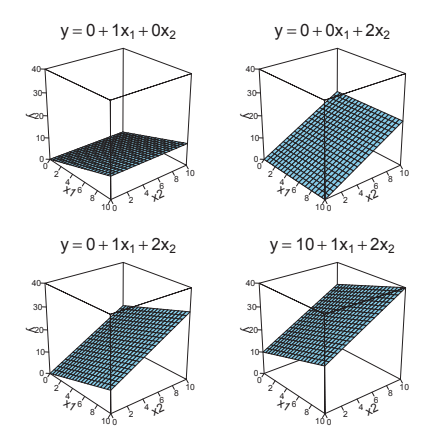
\includegraphics[height=.8\textheight]{img/fig15_2}
\end{figure}
\end{frame}

\begin{frame}
\frametitle{Linear combination of metric predictors (II)}

\textbf{Bilinear function:} $\sim$ polynomial function with no self-interactions:
\begin{align*}
    f(x + a, y) &= f(x, y) + f(a, y) \\
    f(x, y + a) &= f(x, y) + f(x, a) \\
    f(ax, y) &= f(x, ay) = a\cdot f(x, y)\\
\end{align*}

With interactions (conditionally linear):
\begin{align*}
\operatorname{lin}_{\beta}(x) &= \beta_0 + \sum_k^K \beta_k x_k + \sum_j^K \sum_{k=j+1}^K \beta_{jk} x_j x_k \\
\end{align*}

\end{frame}

\begin{frame}
\frametitle{Linear combination of metric predictors (II)}
\begin{figure}
\centering
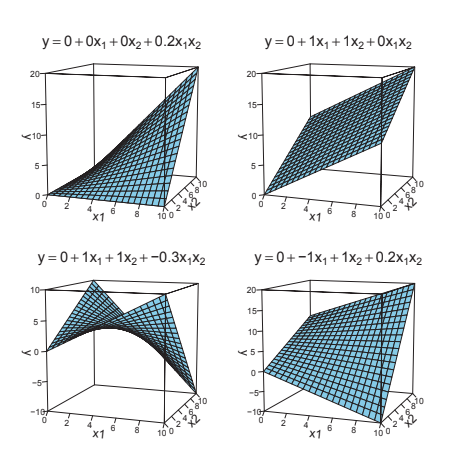
\includegraphics[height=.8\textheight]{img/fig15_3}
\end{figure}
\end{frame}


\begin{frame}
\frametitle{Aside: Notation for linear combinations (I)}
\textbf{Common approach:} write down the power series expansion
\begin{align*}
f(x_1) = \beta_0 + \beta_1 x_1 &= \beta_0 x_1^0 + \beta_1 x_1^1
\end{align*}

\textbf{Works for two variables:}
\begin{align*}
f(x_1, x_2) &= \beta_{00} x_1^0 x_2^0 + \beta_{10} x_1^1 x_2^0 + \beta_{01} x_1^0 x_2^1 + \beta_{11} x_1^1 x_2^1 + \ldots \\
            &= \sum_{i=0}^P \sum_{j=0}^P \beta_{ij} x_1^i x_2^j
\end{align*}

\textbf{Problem:} Scaling to arbitrary dimensions, notation unwieldy:
\begin{align*}
f(\widehat{x}) &= \sum_{i=0}^P \sum_{j=0}^P \sum_{k=0}^P \ldots \left( \beta_{ijk\ldots} x_1^i x_2^j x_3^k\ldots \right)
\end{align*}
\end{frame}

\begin{frame}
\frametitle{Aside: Notation for linear combinations (II)}
\textbf{(One) solution:} Introduce bias in feature vector: $\widehat{x} = <x_1. x_2, \ldots> \rightarrow \widehat{x} = <1, x_1, x_2, \ldots>$:
\begin{align*}
f(x_1) &= \beta_0 + \beta_1 x_1 = \beta_0 x_0 + \beta_1 x_1 : x_0 = 1 \\
f(x_1, x_2) &= \beta_{00} x_0 x_0 + \beta_{01} x_0 x_1 + \beta_{02} x_0 x_2 + \beta_{12} x_1 x_2 \\
            &= \beta_{00} + \beta_{01} x_1 + \beta_{02} x_2 + \beta_{12} x_1 x_2 \\
f(\widehat{x})&= \sum_{i=0}^K \sum_{j=i+1}^K \beta_{ij} x_i x_j : x_0 = 1
\end{align*}

\textbf{Note:} This is a more compact representation of $\operatorname{lin}_{\beta}(x) = \beta_0 + \sum_i^K \beta_i x_i + \sum_i^K\sum_{j=i+1}^K \beta_i x_i x_j$

\textbf{Note:} If $j=i+1$ is changed to $j=i$, self-interactions are taken into consideration (but this violates conditional linearity).

\end{frame}










\begin{frame}
\frametitle{Nominal predictors}

\textbf{One-hot coding:} Each feature is vector (instead of scalar) $\widehat{x} = <0, 0, 1>$

For metric predictors each sample has a number of features:
\begin{align*}
    \begin{matrix}
    \textrm{feature 0} & \textrm{feature 1} & \textrm{feature 2} & \ldots \\
    x_0 & x_1 & x_2 & \ldots
    \end{matrix}
\end{align*}

For nominal predictors each feature is a vector:
\begin{align*}
    \begin{matrix}
    & \textrm{feature 0} & \textrm{feature 1} & \textrm{feature 2} & \ldots \\
    \textrm{category 0} & x_{00} & x_{01} & x_{02} & \ldots \\
    \textrm{category 1} & x_{10} & x_{11} & x_{12} & \ldots \\
    \textrm{category 2} & x_{20} & x_{21} & x_{22} & \ldots \\
    \end{matrix}
\end{align*}

\end{frame}


\begin{frame}
\frametitle{Linear combinations of Nominal predictors}

Linear combination:
\begin{align*}
    lin(\widehat{x}) = \beta_0 + \sum_j \widehat{\beta_j} \cdot \widehat{x}_j
\end{align*}
where $\cdot$ denotes the dot product.

\vspace{1em}
\textbf{Intuition:} Think of $\beta_0$ as population ``average'', and $\beta_j$ as ``average'' of group $j$.

\end{frame}

\begin{frame}
\frametitle{Linear combinations of Nominal predictors}
\begin{figure}
\centering
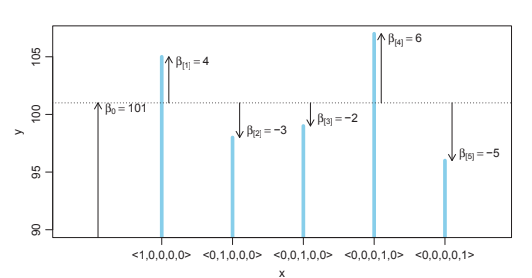
\includegraphics[width=\textwidth]{img/fig15_4}
\end{figure}
\end{frame}

\begin{frame}
\frametitle{Summary Linear Combination}
Form of linear function in GLM for different scale types (of predictor $x$):
\begin{figure}
\centering
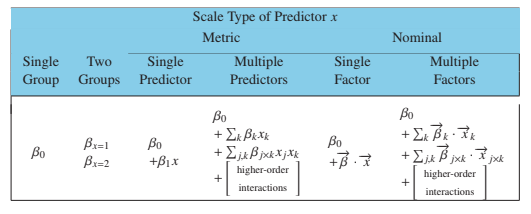
\includegraphics[width=\textwidth]{img/fig15_11}
\end{figure}
\end{frame}

\begin{frame}
\frametitle{Linking from Combined Predictors to (noisy) predicted data}

\begin{align*}
y = f(\operatorname{lin}(x)) \tag{15.11}
\end{align*}

Here $f$ is called the (inverse) link function and converts the combined predictors to an apporopriate output scale.

\begin{align*}
\textrm{Input Space} \overset{\operatorname{lin}}{\rightarrow} \parbox{7em}{\textrm{Combined predictor Space}} \overset{f}{\rightarrow} \textrm{Output Space}
\end{align*}

\begin{table}
\centering
\begin{tabular}{cc}
\textbf{Scale Type} & \textbf{Task} \\
Metric     & Regression \\
Nominal    & Classification
\end{tabular}
\end{table}
\end{frame}


\begin{frame}
\frametitle{Logistic function}
Link function common for classification: the \emph{logistic} function. Unrestricted domain, range $(0, 1)$. $\operatorname{logistic(x) = 1/ (1+\exp\,(-x))}$
\begin{figure}
\centering
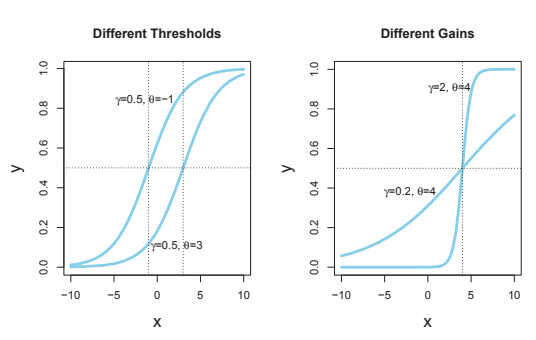
\includegraphics[width=0.6\textwidth]{img/fig15_6}
\end{figure}

Note: Another reasonable choice: $\Phi$, the cumulative normal distribution (convenicent for e.g. ordinal data).
\end{frame}

\begin{frame}
\frametitle{Noisy output}
\begin{columns}
\column{.5\textwidth}
\begin{align*}
y &\sim \operatorname{pdf}(\mu, [\textrm{parameters}]) \\
\mu &= f(\operatorname{lin}(x))
\end{align*}

If $f$ is indentity: Linear regression.
\column{.5\textwidth}
\begin{figure}
\centering
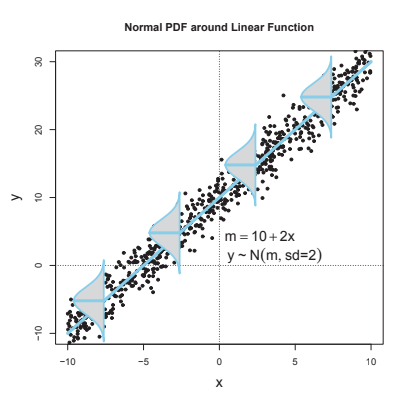
\includegraphics[width=\textwidth]{img/fig15_9_1}
\end{figure}
\end{columns}
\end{frame}

\begin{frame}
\frametitle{Noisy output (II)}
\begin{columns}
\column{.5\textwidth}
\begin{align*}
y &\sim \operatorname{pdf}(\mu, [\textrm{parameters}]) \\
\mu &= f(\operatorname{lin}(x))
\end{align*}

If $f$ is logistic: Logistic regression. (Special case of binary classification).
\column{.5\textwidth}
\begin{figure}
\centering
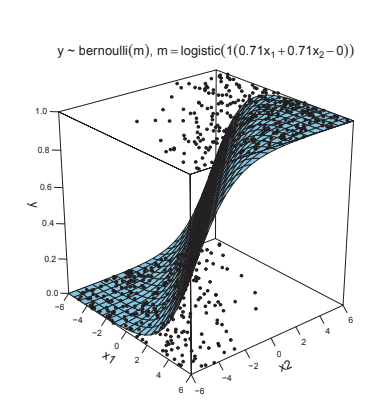
\includegraphics[width=\textwidth]{img/fig15_10}
\end{figure}
\end{columns}
\end{frame}


\begin{frame}
\frametitle{Typical distributions and link functions}
\begin{figure}
\centering
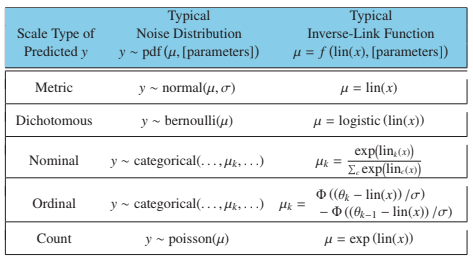
\includegraphics[width=\textwidth]{img/fig15_12}
\end{figure}
\end{frame}

\begin{frame}
\frametitle{Aside: Link function and loss function}

Minimising the \emph{Bayesian risk} w.r.t. a given loss function yields a particular \emph{invertible link function}. Can this be considered regression on likelihood?

\begin{align*}
I[f] &= \int_{X \times Y} \mathcal{L}(f(x), y)p(x, y)\, dx\, dy \\
     &= \int_{X} \int_{Y} \phi(y f(x))p(y|x)p(x)\, dx\, dy \\
     &= \int_{X} \left( \phi(f(x))p(y=1|x) + \phi(-f(x))p(y=-1|x) \right) p(x)\, dx\ \\
     &= \int_{X} \left( (\phi(f(x)) - \phi(-f(x)))p(y=1|x) + \phi(-f(x)) \right)p(x)\, dx\ \\
\end{align*}

\end{frame}

\begin{frame}
\frametitle{Aside: Link function and loss function}

\textbf{Note:} $p(y=\mathrm{A}|\widehat{x}) = \eta = f^{-1}(v) = 1 - p(y=\mathrm{B}|\widehat{x})$. I.e. binary classification given some input variable $x$.

\begin{table}
\begin{tabular}{ccccc}
\textbf{Loss name} & $\phi(v)$ & $C(\eta)$ & $f^{-1}(v)$ & $f(v)$ \\
Exponential        & $e^{-v}$  \\
Logistic           & $\frac{\log (1 + e^{-v})}{\log(2)}$ & - & $\frac{e^v}{1 + e^v}$ & $\log(\frac{\eta}{1 - \eta})$\\
Square             & $$ & - & $$ \\
Savage             & $$ & - & $$ \\
Tangent            & $$ & - & $$ \\

\end{tabular}
\end{table}

\textcolor{gray}{\small\url{en.wikipedia.org/wiki/Loss_functions_for_classification}}
\end{frame}

\end{document} 